\documentclass[multi=tikzpicture,border=1pt]{standalone}
\usepackage[svgnames]{xcolor}
\usepackage{pgf}
\usepackage{tikz}
\usetikzlibrary{shapes,arrows}

\usepackage{fontspec}
\setmainfont{Myriad Pro}

\definecolor{cbSkyblue}{RGB}{86,180,233}
\definecolor{cbGreen}{RGB}{0,158,115}
\definecolor{cbYellow}{RGB}{240,228,66}
\definecolor{cbPurple}{RGB}{204,121,167}%DeepPink
\definecolor{monokai}{RGB}{39,40,34}
\begin{document}

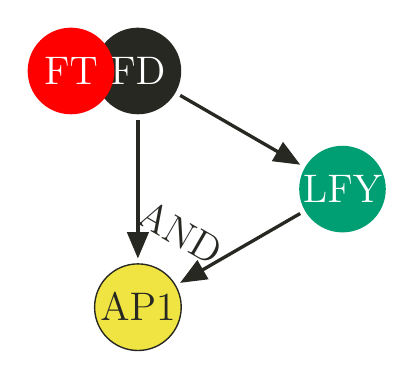
\begin{tikzpicture}[auto, shorten <=2pt, shorten >=2pt]%
  \tikzset{normal arrow/.style={draw,-triangle 45,very thick,monokai}}
  \tikzstyle{every node}=[draw=none, text=white, circle, minimum size=1.1cm, outer sep=0pt, inner sep=0pt, font=\Large]

  \node[fill=monokai] at (0,0) (FD) {FD};
  \node[fill=cbGreen] at (-30:3cm) (LFY) {LFY};
  \node[fill=cbYellow,draw=monokai,line width=0.5pt,text=monokai] at (270:3cm) (AP1)  {AP1};
  \node[fill=red, node distance = 0.85cm] (FT) [left of=FD] {FT};

  \path[normal arrow] (FD) edge   (LFY);
  \path[normal arrow] (LFY) -- node[yshift=-0.1cm, left=0.25cm, rotate=330, text=monokai] {AND} (AP1);
  \path[normal arrow]  (FD) edge  (AP1);
\end{tikzpicture}

\newpage

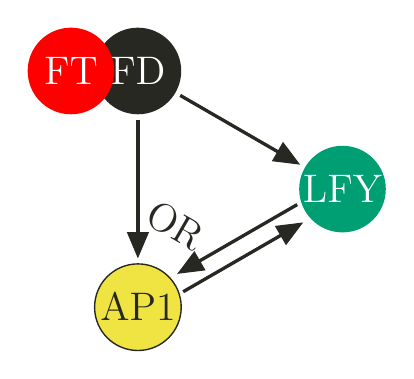
\begin{tikzpicture}[auto, shorten <=2pt, shorten >=2pt]%
  \tikzset{normal arrow/.style={draw,-triangle 45,very thick,monokai}}
  \tikzstyle{every node}=[draw=none, text=white, circle, minimum size=1.1cm, outer sep=0pt, inner sep=0pt, font=\Large]

    \node[fill=monokai] at (0,0) (FD) {FD};
  \node[fill=cbGreen] at (-30:3cm) (LFY) {LFY};
  \node[fill=cbYellow,draw=monokai,line width=0.5pt,text=monokai] at (270:3cm) (AP1)  {AP1};
  \node[fill=red, node distance = 0.85cm] (FT) [left of=FD] {FT};

  % \node[fill=cbGreen] at (0,0) (FD) {FD};
  % \node[fill=cbSkyblue] at (-30:3cm) (LFY) {LFY};
  % \node[fill=red] at (270:3cm) (AP1)  {AP1};
  % \node[fill=cbPurple, node distance = 0.85cm] (FT) [left of=FD] {FT};

  \path[normal arrow] (FD) edge   (LFY);
  \path[normal arrow,transform canvas={yshift=+0.75ex, xshift=-0.25ex}] (LFY) -- node[yshift=-0.1cm, left=0.3cm, rotate=330, text=monokai] {OR} (AP1);
  \path[normal arrow,transform canvas={yshift=-0.75ex, xshift=+0.25ex}] (AP1) edge (LFY);
  \path[normal arrow]  (FD) edge  (AP1);
\end{tikzpicture}

\newpage

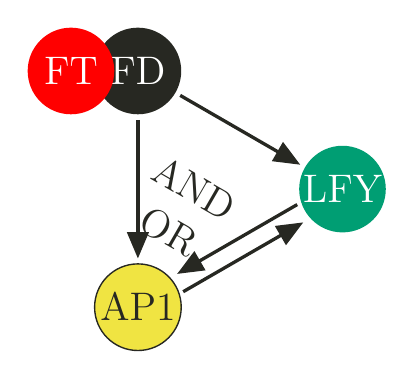
\begin{tikzpicture}[auto, shorten <=2pt, shorten >=2pt]%
  \tikzset{normal arrow/.style={draw,-triangle 45,very thick,monokai}}
  \tikzstyle{every node}=[draw=none, text=white, circle, minimum size=1.1cm, outer sep=0pt, inner sep=0pt, font=\Large]

  \node[fill=monokai] at (0,0) (FD) {FD};
  \node[fill=cbGreen] at (-30:3cm) (LFY) {LFY};
  \node[fill=cbYellow,draw=monokai,line width=0.5pt,text=monokai] at (270:3cm) (AP1)  {AP1};
  \node[fill=red, node distance = 0.85cm] (FT) [left of=FD] {FT};
  
  % \node[fill=cbGreen] at (0,0) (FD) {FD};
  % \node[fill=cbSkyblue] at (-30:3cm) (LFY) {LFY};
  % \node[fill=red] at (270:3cm) (AP1)  {AP1};
  % \node[fill=cbPurple, node distance = 0.85cm] (FT) [left of=FD] {FT};

  \path[normal arrow] (FD) edge   (LFY);
  \path[normal arrow,transform canvas={yshift=+0.75ex, xshift=-0.25ex}] (LFY) -- node[yshift=-0.0cm,left=0.06cm, rotate=330, text=monokai,align=center] {AND\\ OR} (AP1);
  \path[normal arrow,transform canvas={yshift=-0.75ex, xshift=+0.25ex}] (AP1) edge (LFY);
  \path[normal arrow]  (FD) edge  (AP1);
\end{tikzpicture}

\newpage

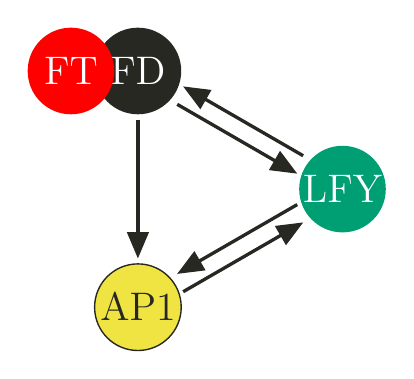
\begin{tikzpicture}[auto, shorten <=2pt, shorten >=2pt]%
  \tikzset{normal arrow/.style={draw,-triangle 45,very thick,monokai}}
  \tikzstyle{every node}=[draw=none, text=white, circle, minimum size=1.1cm, outer sep=0pt, inner sep=0pt, font=\Large]

  \node[fill=monokai] at (0,0) (FD) {FD};
  \node[fill=cbGreen] at (-30:3cm) (LFY) {LFY};
  \node[fill=cbYellow,draw=monokai,line width=0.5pt,text=monokai] at (270:3cm) (AP1)  {AP1};
  \node[fill=red, node distance = 0.85cm] (FT) [left of=FD] {FT};
  % \node[fill=cbGreen] at (0,0) (FD) {FD};
  % \node[fill=cbSkyblue] at (-30:3cm) (LFY) {LFY};
  % \node[fill=red] at (270:3cm) (AP1)  {AP1};
  % \node[fill=cbPurple, node distance = 0.85cm] (FT) [left of=FD] {FT};

  \path[normal arrow,transform canvas={yshift=-0.75ex, xshift=-0.25ex}] (FD) edge   (LFY);
  \path[normal arrow,transform canvas={yshift=+0.75ex, xshift=-0.25ex}] (LFY) edge (AP1);
  \path[normal arrow,transform canvas={yshift=-0.75ex, xshift=+0.25ex}] (AP1) edge (LFY);
  \path[normal arrow]  (FD) edge  (AP1);
  \path[normal arrow,transform canvas={yshift=+0.75ex, xshift=+0.25ex}]  (LFY) edge  (FD);
\end{tikzpicture}

\newpage

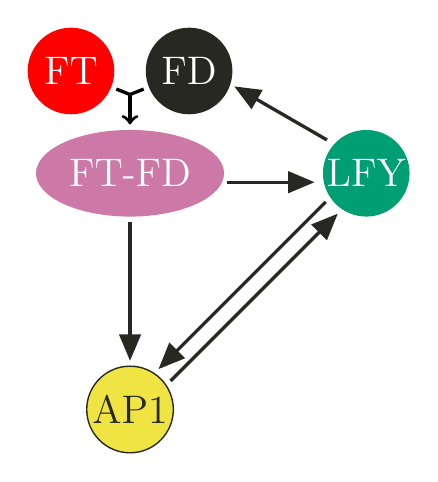
\begin{tikzpicture}[auto, shorten <=2pt, shorten >=2pt]%
  \tikzset{normal arrow/.style={draw,-triangle 45,very thick,monokai}}
  \tikzstyle{every node}=[draw=none, text=white, minimum size=1.1cm, outer sep=0pt, inner sep=0pt, font=\Large]

  \coordinate (m1) at (90:10mm);
  \node[fill=monokai, circle] at (60:15mm) (FD) {FD};
  \node[fill=cbGreen, circle] at (0:3cm) (LFY) {LFY};
  \node[fill=cbYellow, circle,draw=monokai,line width=0.5pt,text=monokai] at (270:3cm) (AP1)  {AP1};
  \node[fill=red, circle, node distance = 15mm] (FT) [left of=FD] {FT};
  \node[ellipse,fill=cbPurple, inner xsep=2pt] at (0,0) (FTFD) {FT-FD};
  
  \path[<-,draw, very thick, shorten >=0pt] (FTFD) edge (m1);
  \path[draw, very thick, shorten >=0pt] (FT) edge (m1);
  \path[draw, very thick, shorten >=0pt] (FD) edge (m1);
  
  %\path[very thick] (FT) edge (FD);
  \path[normal arrow,transform canvas={yshift=-0.75ex, xshift=-0.25ex}] (FTFD) edge   (LFY);
  \path[normal arrow,transform canvas={yshift=+0.5ex, xshift=-0.5ex}] (LFY) edge (AP1);
  \path[normal arrow,transform canvas={yshift=-0.5ex, xshift=+0.5ex}] (AP1) edge (LFY);  
  \path[normal arrow]  (FTFD) edge  (AP1);
  \path[normal arrow,transform canvas={yshift=+0.75ex, xshift=+0.25ex}]  (LFY) edge  (FD);

\end{tikzpicture}

\newpage

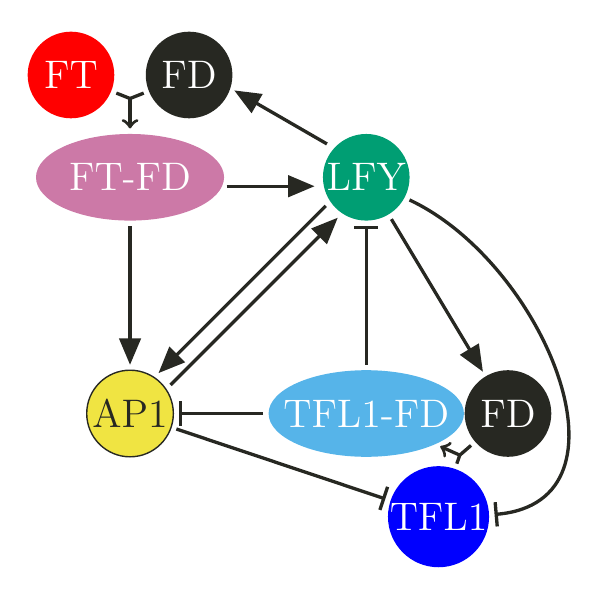
\begin{tikzpicture}[auto, shorten <=2pt, shorten >=2pt]%
  \tikzset{normal arrow/.style={draw,-triangle 45,very thick,monokai}}
  \tikzstyle{every node}=[draw=none, text=white, minimum size=1.1cm, outer sep=0pt, inner sep=0pt, font=\Large]
  \tikzstyle{every path}=[monokai]

  \coordinate (m1) at (90:10mm);
  \node[fill=monokai, circle] at (60:15mm) (FD) {FD};
  \node[fill=cbGreen, circle] at (0:3cm) (LFY) {LFY};
  \node[fill=cbYellow, circle,draw=monokai,line width=0.5pt,text=monokai] at (270:3cm) (AP1)  {AP1};
  \node[fill=red, circle, node distance = 15mm] (FT) [left of=FD] {FT};
  \node[ellipse,fill=cbPurple, inner xsep=2pt] at (0,0) (FTFD) {FT-FD};

  \node[ellipse,fill=cbSkyblue, node distance = 30mm, inner xsep=-5pt] (TFL1FD) [right of=AP1] {TFL1-FD};
  \node[fill=monokai, circle] (FD2) [right of=TFL1FD, node distance = 18mm] {FD};
  \node[fill=blue, circle] (TFL1) at ([shift={(TFL1FD)}] 305:16mm) {TFL1};
  \coordinate (m2) at ([shift={(TFL1FD)}] 336:13mm);

  \path[<-,draw, very thick, shorten >=0pt] (FTFD) edge (m1);
  \path[draw, very thick, shorten >=0pt] (FT) edge (m1);
  \path[draw, very thick, shorten >=0pt] (FD) edge (m1);
  %\path[draw,very thick] (FT) --coordinate[midway](m1) (FD);
  \path[normal arrow,transform canvas={yshift=-0.75ex, xshift=-0.25ex}] (FTFD) edge   (LFY);
  %\path[draw, very thick, shorten >=0pt] (FTFD) -- (m1); 
  \path[normal arrow,transform canvas={yshift=+0.5ex, xshift=-0.5ex}] (LFY) edge (AP1);
  \path[normal arrow,transform canvas={yshift=-0.5ex, xshift=+0.5ex}] (AP1) edge (LFY);
  \path[normal arrow]  (FTFD) edge  (AP1);
  \path[normal arrow,transform canvas={yshift=+0.75ex, xshift=+0.25ex}]  (LFY) edge  (FD);
  \path[-|, very thick, draw]  (AP1) edge (TFL1);

  \pgfresetboundingbox% Stupid hack to get tight figure
  \useasboundingbox (-1.3,-4.9) rectangle (5.5,1.9);%Curves prob have Bezier points outside causing unneeded white space
  \path[very thick, draw]  (LFY) edge[bend left, -|,in=80, out=50, looseness=1.2] (TFL1);
  \path[normal arrow]  (LFY) edge (FD2);
  \path[-|, very thick, draw]  (TFL1FD) edge (LFY);
  \path[-|, very thick, draw]  (TFL1FD) edge (AP1);
  %\path[very thick, draw] (TFL1) --coordinate[midway](m2) (FD2);
  %\path[draw, very thick, shorten >=0pt] (TFL1FD) -- (m2);
  \path[<-,draw, very thick, shorten >=0pt] (TFL1FD) edge (m2);
  \path[draw, very thick, shorten >=0pt] (TFL1) edge (m2);
  \path[draw, very thick, shorten >=0pt] (FD2) edge (m2);
\end{tikzpicture}

\newpage

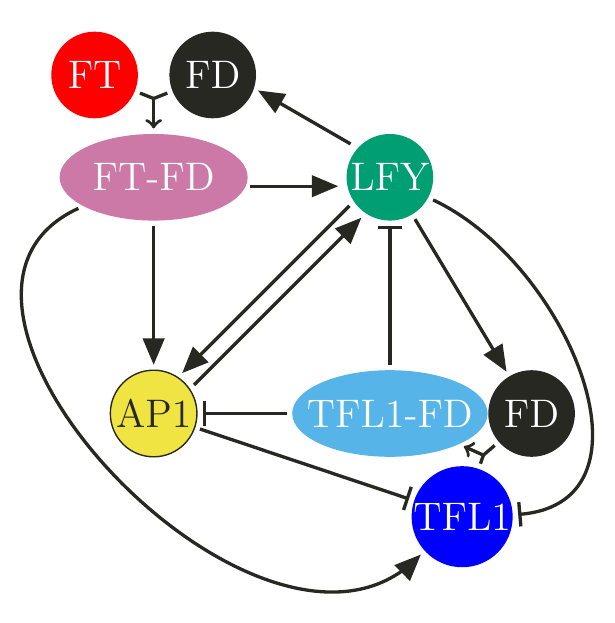
\begin{tikzpicture}[auto, shorten <=2pt, shorten >=2pt]%
  \tikzset{normal arrow/.style={draw,-triangle 45,very thick,monokai}}
  \tikzstyle{every node}=[draw=none, text=white, minimum size=1.1cm, outer sep=0pt, inner sep=0pt, font=\Large]
  \tikzstyle{every path}=[monokai]

  \coordinate (m1) at (90:10mm);
  \node[fill=monokai, circle] at (60:15mm) (FD) {FD};
  \node[fill=cbGreen, circle] at (0:3cm) (LFY) {LFY};
  \node[fill=cbYellow, circle,draw=monokai,line width=0.5pt,text=monokai] at (270:3cm) (AP1)  {AP1};
  \node[fill=red, circle, node distance = 15mm] (FT) [left of=FD] {FT};
  \node[ellipse,fill=cbPurple, inner xsep=2pt] at (0,0) (FTFD) {FT-FD};

  \node[ellipse,fill=cbSkyblue, node distance = 30mm, inner xsep=-5pt] (TFL1FD) [right of=AP1] {TFL1-FD};
  \node[fill=monokai, circle] (FD2) [right of=TFL1FD, node distance = 18mm] {FD};
  \node[fill=blue, circle] (TFL1) at ([shift={(TFL1FD)}] 305:16mm) {TFL1};
  \coordinate (m2) at ([shift={(TFL1FD)}] 336:13mm);

  \path[<-,draw, very thick, shorten >=0pt] (FTFD) edge (m1);
  \path[draw, very thick, shorten >=0pt] (FT) edge (m1);
  \path[draw, very thick, shorten >=0pt] (FD) edge (m1);
  %\path[draw,very thick] (FT) --coordinate[midway](m1) (FD);
  \path[normal arrow,transform canvas={yshift=-0.75ex, xshift=-0.25ex}] (FTFD) edge   (LFY);
  %\path[draw, very thick, shorten >=0pt] (FTFD) -- (m1); 
  \path[normal arrow,transform canvas={yshift=+0.5ex, xshift=-0.5ex}] (LFY) edge (AP1);
  \path[normal arrow,transform canvas={yshift=-0.5ex, xshift=+0.5ex}] (AP1) edge (LFY);
  \path[normal arrow]  (FTFD) edge  (AP1);
  \path[normal arrow,transform canvas={yshift=+0.75ex, xshift=+0.25ex}]  (LFY) edge  (FD);
  \path[-|, very thick, draw]  (AP1) edge (TFL1);
  \pgfresetboundingbox% Stupid hack to get tight figure
  \useasboundingbox (-1.6,-5.3) rectangle (5.5,1.9);%Curves prob have Bezier points outside causing unneeded white space
  \path[very thick, draw]  (LFY) edge[bend left, -|,in=80, out=50, looseness=1.2] (TFL1);
  \path[normal arrow]  (LFY) edge (FD2);
  \path[-|, very thick, draw]  (TFL1FD) edge (LFY);
  \path[-|, very thick, draw]  (TFL1FD) edge (AP1);
  %\path[very thick, draw] (TFL1) --coordinate[midway](m2) (FD2);
  %\path[draw, very thick, shorten >=0pt] (TFL1FD) -- (m2);
  \path[<-,draw, very thick, shorten >=0pt] (TFL1FD) edge (m2);
  \path[draw, very thick, shorten >=0pt] (TFL1) edge (m2);
  \path[draw, very thick, shorten >=0pt] (FD2) edge (m2);
  \path[normal arrow]  (FTFD) edge[bend right,in=270, out=250, looseness=1.2]  (TFL1);
\end{tikzpicture}
\end{document}
